\documentclass[10pt,twocolumn,letterpaper]{article}

\usepackage[letterpaper,top=0.85in,bottom=0.9in,left=0.65in,right=0.65in,columnsep=0.28in]{geometry}
\usepackage{amsmath}
\usepackage[T1]{fontenc}
\usepackage{stix2}                 % body and math font (as in the CSEN 140 report)
\usepackage[scaled=0.92]{helvet}   % sans font for title, headings and captions
\usepackage{microtype}
\usepackage{graphicx}
\usepackage{booktabs}
\usepackage{tabularx}
\usepackage{caption}
\usepackage{enumitem}
\usepackage{xcolor}
\usepackage{titlesec}
\usepackage{fancyhdr}
\usepackage{lastpage}
\usepackage[colorlinks=true,linkcolor=blue!50!black,citecolor=blue!50!black,urlcolor=blue!50!black]{hyperref}

\definecolor{titleblue}{RGB}{24,64,120}
\graphicspath{{figures/}}
\setlist{itemsep=2pt,topsep=4pt,leftmargin=*}
\captionsetup{font=small,labelfont={bf,sf},labelsep=period}
\newcommand{\code}[1]{\texttt{\detokenize{#1}}}

% headings: sans, numbered "1. Abstract", "4.1. ..."
\titleformat{\section}{\sffamily\bfseries\large\color{titleblue}}{\thesection.}{0.5em}{}
\titleformat{\subsection}{\sffamily\bfseries\normalsize}{\thesubsection.}{0.5em}{}
\titleformat{\paragraph}[runin]{\sffamily\bfseries\small}{}{0pt}{}
\titlespacing*{\section}{0pt}{12pt}{6pt}
\titlespacing*{\subsection}{0pt}{9pt}{4pt}
\titlespacing*{\paragraph}{0pt}{6pt}{0.5em}

% let full-width figures share pages with text
\renewcommand{\topfraction}{0.9}
\renewcommand{\dbltopfraction}{0.9}
\renewcommand{\textfraction}{0.1}
\renewcommand{\floatpagefraction}{0.8}
\renewcommand{\dblfloatpagefraction}{0.8}
\setcounter{topnumber}{3}
\setcounter{dbltopnumber}{3}

\newcommand{\reporttitle}{Where Help Is Far Away: Fire-Station Distance, Wildfire Growth, and Types of Under-Served Areas in the United States}
\newcommand{\shorttitle}{Where Help Is Far Away: Fire-Station Distance and Wildfire Growth}

\pagestyle{fancy}
\fancyhf{}
\renewcommand{\headrulewidth}{0pt}
\fancyhead[R]{\footnotesize\itshape\shorttitle}
\fancyfoot[L]{\footnotesize\sffamily\textbf{\thepage}\quad CSEN 281}
\fancyfoot[R]{\footnotesize\sffamily Santa Clara University\quad\textbf{October, 2026}\quad Milestone 1 Report}
\fancypagestyle{first}{%
  \fancyhf{}
  \fancyfoot[L]{\footnotesize\sffamily CSEN 281}
  \fancyfoot[R]{\footnotesize\sffamily Santa Clara University\quad\textbf{October, 2026}\quad Milestone 1 Report\quad\textbf{1--\pageref{LastPage}}}%
}

\begin{document}
\twocolumn[{%
\begin{flushleft}
{\sffamily\bfseries\small CSEN 281 - Capstone Milestone 1 Report}\par\vspace{8pt}
{\sffamily\bfseries\LARGE\color{titleblue}\reporttitle\par}\vspace{8pt}
{\sffamily\bfseries\normalsize Quan Do\textsuperscript{a} and Nandingoo Erdenebat\textsuperscript{b}\par}\vspace{6pt}
{\footnotesize\itshape \textsuperscript{a}CSEN - qldo@scu.edu\\
\textsuperscript{b}CSEN -nerdenebat@scu.edu\par}
\end{flushleft}
\vspace{14pt}
}]
\thispagestyle{first}

\section{Abstract}
The Fire Program Analysis Fire-Occurrence Database (FPA-FOD) records 2.66 million US wildfires from 1992 to 2024, but it says nothing about where firefighting resources are. We join it with the HIFLD Fire and EMS Stations layer (52{,}057 stations) and compute, for every fire, the great-circle distance to the nearest station. Exploratory analysis shows that the share of fires growing to 100 acres or more rises from 0.75\% for fires within 2~km of a station to 16.9\% for fires more than 40~km away. The trend holds within every region and cause class and in recent years. A logistic model puts it at 1.80 times the odds of a large fire per doubling of distance after adjusting for state, land owner, month and year. The effect is above 1 in every region, owner group, cause class and year, and it shrinks but never disappears when up to 75\% of stations are removed at random. 58\% of fires start within 5~km of a station, but those fires account for only 14\% of the area burned. These findings motivate two questions. \textbf{(1, supervised)} How much does station distance raise the chance that a fire becomes large, after accounting for where, when and why it started? An untuned gradient-boosted model on a strict 2019--2024 hold-out improves from 0.119 to 0.153 PR-AUC when distance is added, and a discovery-time model without cause reaches 0.163 with distance and the number of nearby stations. \textbf{(2, unsupervised)} Among under-served areas, what distinct types exist, and what help would each need? Clustering 2{,}271 under-served grid cells, which hold 42\% of burned acres, gives four interpretable regimes that separate cleanly on a held-out cause variable and are fairly stable under bootstrap resampling (ARI 0.88). A coverage experiment shows that adding stations alone closes little of the gap. This report documents the data, the EDA and the methods planned for Milestones 2 and 3.


%=====================================================================
\section{Introduction}
%=====================================================================
Most wildfires are caught small. Whether a fire stays small depends on how quickly it is found and how quickly crews reach it. Response time is not recorded in the FPA-FOD, but distance to the nearest fire station is a measurable proxy for it once station locations are added. If fires far from stations reliably grow larger, that distance is a lever planners can act on: where to add stations, where to pre-position crews, and where stations will not help and other tools (aircraft, detection, fuel treatment) are needed.

This project asks two connected questions. The supervised question measures \emph{how much} distance matters for a single fire. The unsupervised question moves from fires to \emph{places}: it groups the areas that are far from help into types, so that each type can be matched with the kind of help that fits it.

All EDA is in one notebook, \code{milestone1_eda.ipynb}. Part~A profiles the wildfire table on its own; this report summarises those data-quality findings and focuses on Part~B, which adds the station data.

%=====================================================================
\section{Research Questions}
%=====================================================================
\begin{description}[leftmargin=0pt]
\item[RQ1 (supervised, classification).] \emph{How much does distance to the nearest fire station raise the probability that a wildfire becomes large ($\geq$100 acres), after accounting for where, when and why it started?}
\item[RQ2 (unsupervised, clustering).] \emph{Among areas that have fires but no station nearby, what distinct types exist, and what kind of help would each type need?}
\end{description}
RQ1 tests whether distance matters at all. RQ2 explains why a single fix, more stations everywhere, does not work, and suggests which fix suits which area.

%=====================================================================
\section{Data}
%=====================================================================
\subsection{FPA-FOD, 7th edition}
The FPA-FOD \cite{short2026} (\code{FPA_FOD_20260615.sqlite}) holds 2{,}661{,}383 geo-referenced wildfires from 1992--2024, compiled from federal, state, tribal and local reporting systems. We use location (\code{LATITUDE}, \code{LONGITUDE}, \code{STATE}), timing (\code{DISCOVERY_DATE}, \code{CONT_DATE}), final size (\code{FIRE_SIZE}), cause (\code{NWCG_CAUSE_CLASSIFICATION}, \code{NWCG_GENERAL_CAUSE}) and land owner (\code{OWNER_DESCR}).

\subsection{Why a second dataset is needed}
Both questions depend on where firefighting resources are, and the FPA-FOD does not record that. \code{NWCG_REPORTING_UNIT_NAME} names the reporting office but has no coordinates. The exact points that hold hundreds of fires are reporting offices, not stations. Table~\ref{tab:datasets} lists the options we considered.

\begin{table*}[t]
\centering\small
\caption{External datasets considered.}
\label{tab:datasets}
\begin{tabularx}{\textwidth}{@{}lXX@{}}
\toprule
Dataset & What it adds & Decision \\
\midrule
HIFLD Fire \& EMS Stations \cite{hifld} & 52k station points, national & \textbf{Used} as the station layer \\
HIFLD Hospitals & hospital locations & Not used: FPA-FOD has no injury or evacuation outcome to link to \\
OpenStreetMap \code{amenity=fire_station} & crowd-sourced stations & Planned completeness cross-check \\
USFS / BLM / CAL FIRE station lists & wildland stations & No single national download; noted as a limitation \\
gridMET weather, LANDFIRE fuels/terrain & fire-behaviour controls & Future work (large raster joins) \\
\bottomrule
\end{tabularx}
\end{table*}

\subsection{HIFLD Fire and EMS Stations}
The station layer \cite{hifld} is produced by the USGS (The National Map, feature code 74026) and distributed through DHS HIFLD Open. We use the copy archived on DataLumos (project 239161). It contains 52{,}057 points across 56 states and territories, with no missing names and 7 duplicated coordinates. It is stored in \code{fire_station_data/}. Three properties matter for interpretation:
\begin{itemize}
\item \textbf{Snapshot, not history:} 93\% of records were loaded in 2015--2023, so older fires are matched against today's stations.
\item \textbf{Mostly structural stations:} only 302 names (0.6\%) identify a wildland agency (CAL FIRE, USFS, BLM, state forestry).
\item \textbf{Uneven rural completeness}, as noted by the producer.
\end{itemize}

%=====================================================================
\section{Exploratory Data Analysis}
%=====================================================================
The notebook has two parts. Part~A (this subsection and the next) profiles the wildfire table on its own; Part~B (the rest of this section) adds the station data and does the EDA for each question.

\subsection{Data quality}
\begin{itemize}
\item \textbf{Missingness depends on who reported the fire} (Figure~\ref{fig:missing}). Discovery time is missing for 31\% of fires, containment date for 37\%, land owner for 40\% and cause for 26\%. Federal records are nearly complete, while non-federal records lack 43--60\% of these fields. We therefore do not drop rows with a missing containment date. Doing so removes 37.5\% of the data and skews it toward federal fires (20.3\% $\rightarrow$ 31.5\%) and lightning fires (13.4\% $\rightarrow$ 18.2\%).
\item \textbf{Reporting changed in 2020--21.} After 2020 almost every record comes from the interagency system, so \code{SOURCE_SYSTEM_TYPE} effectively encodes the year and is excluded. The share of labelled fires coded ``Other causes'' jumps from about 1\% to 33\% in 2021.
\item \textbf{Values are rounded by hand.} Discovery times pile up on :00 and :30. The values 0.1, 1 and 0.5 acres make up over 40\% of fires. About 7\% of coordinates have two or fewer decimals ($\gtrsim$1~km error). We therefore model a binary size threshold rather than raw acres.
\end{itemize}

\begin{figure}[tb]
\centering
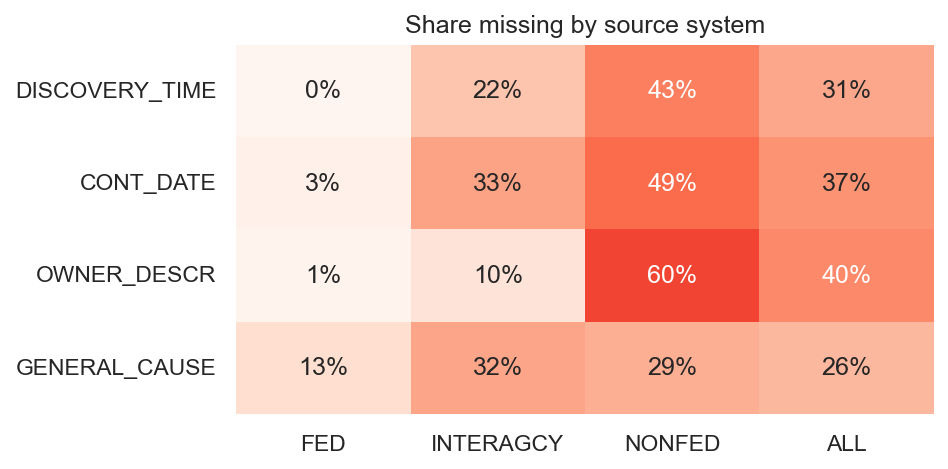
\includegraphics[width=\columnwidth]{missingness.png}
\caption{Share of missing values by field and source system. Missingness tracks the reporting agency, not the fire.}
\label{fig:missing}
\end{figure}

\subsection{When, where and how big fires are}
\begin{itemize}
\item \textbf{Season and cause are linked} (Figure~\ref{fig:season}). 77.8\% of lightning fires start in June--August, while 37.3\% of human fires start in February--April (debris burning before green-up), with a spike on July~4. People-driven causes rise at weekends; lightning is flat across the week. Lightning fires are usually discovered later in the day (16:00 vs.\ 14:00). Season, weekday and cause therefore enter RQ1 as controls.
\item \textbf{Fire counts and burned area are in different places.} Most fires start in the East and Southeast, near people, while most land burns in the West and Alaska (AK 41.0~M acres, CA 25.6~M, ID 18.1~M). Lightning causes most fires in the interior West and under 10\% east of the Plains. Location is a key control for RQ1, and this gap between fires and burned land is what RQ2 is about.
\item \textbf{Size is extremely skewed} (Figure~\ref{fig:size}). Class~G fires (5{,}000+ acres) are 0.21\% of fires but 75.4\% of acres; classes A and B are 86\% of fires but almost no area. Lightning causes 13.4\% of fires but 57.4\% of acres. RQ1 therefore predicts a yes/no target (100+ acres) and RQ2 uses log-scaled size features.
\end{itemize}

\begin{figure*}[t]
\centering
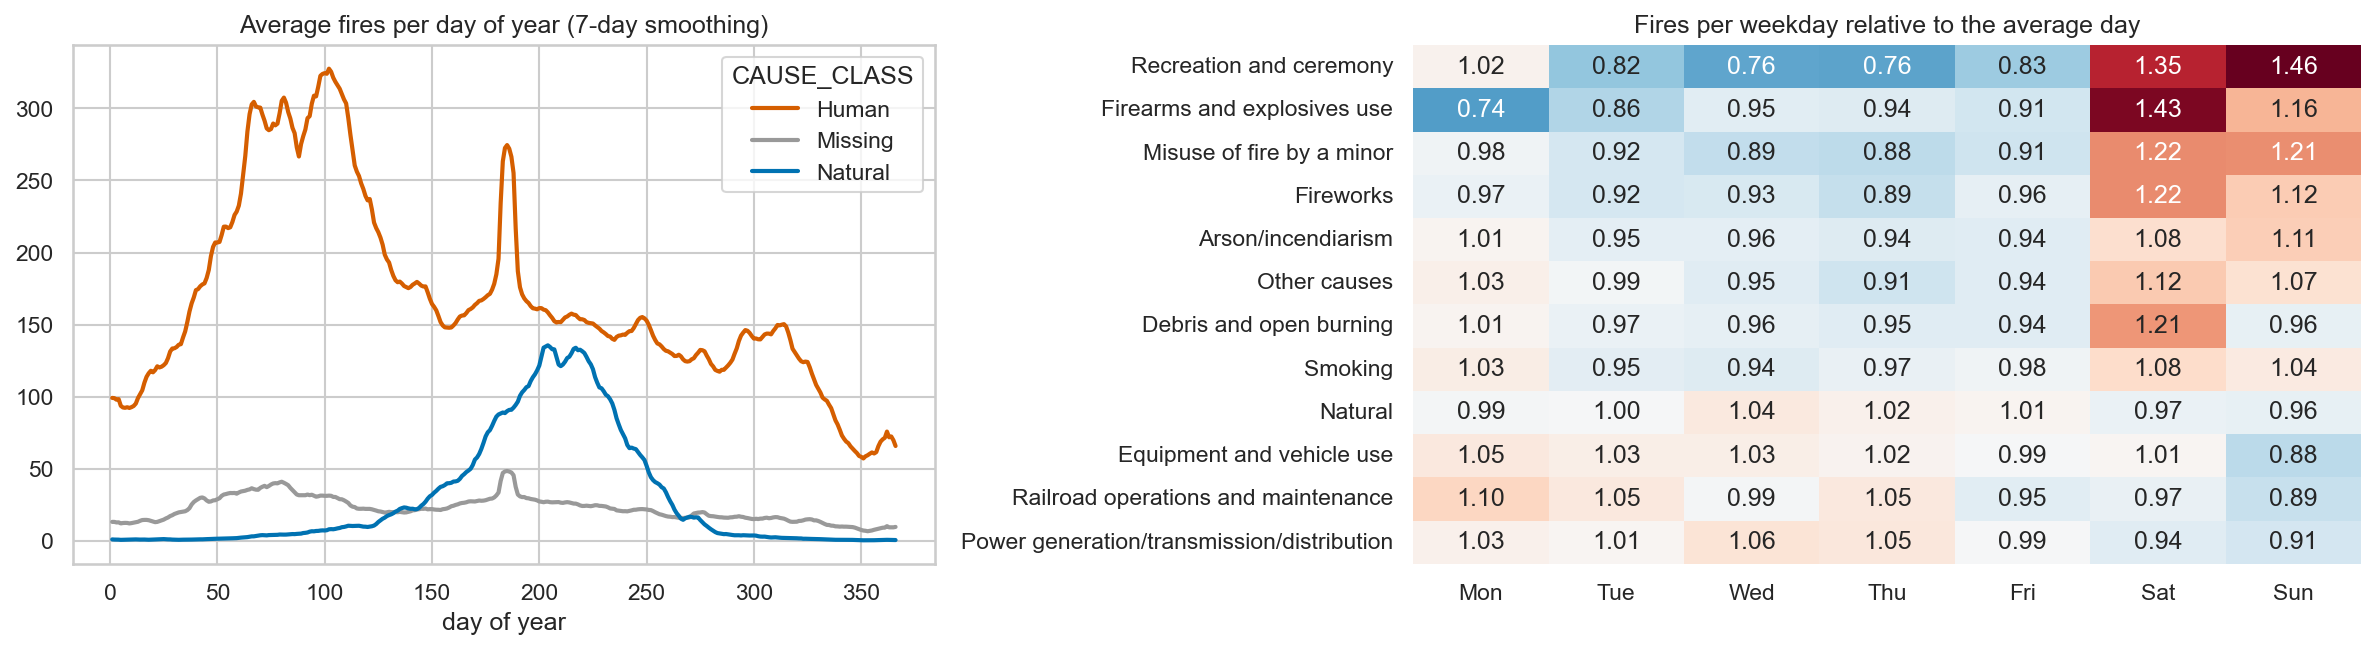
\includegraphics[width=\textwidth]{seasonality.png}
\caption{Left: average fires per day of year by cause class. Right: fires per weekday relative to the average day, by cause.}
\label{fig:season}
\end{figure*}

\begin{figure*}[t]
\centering
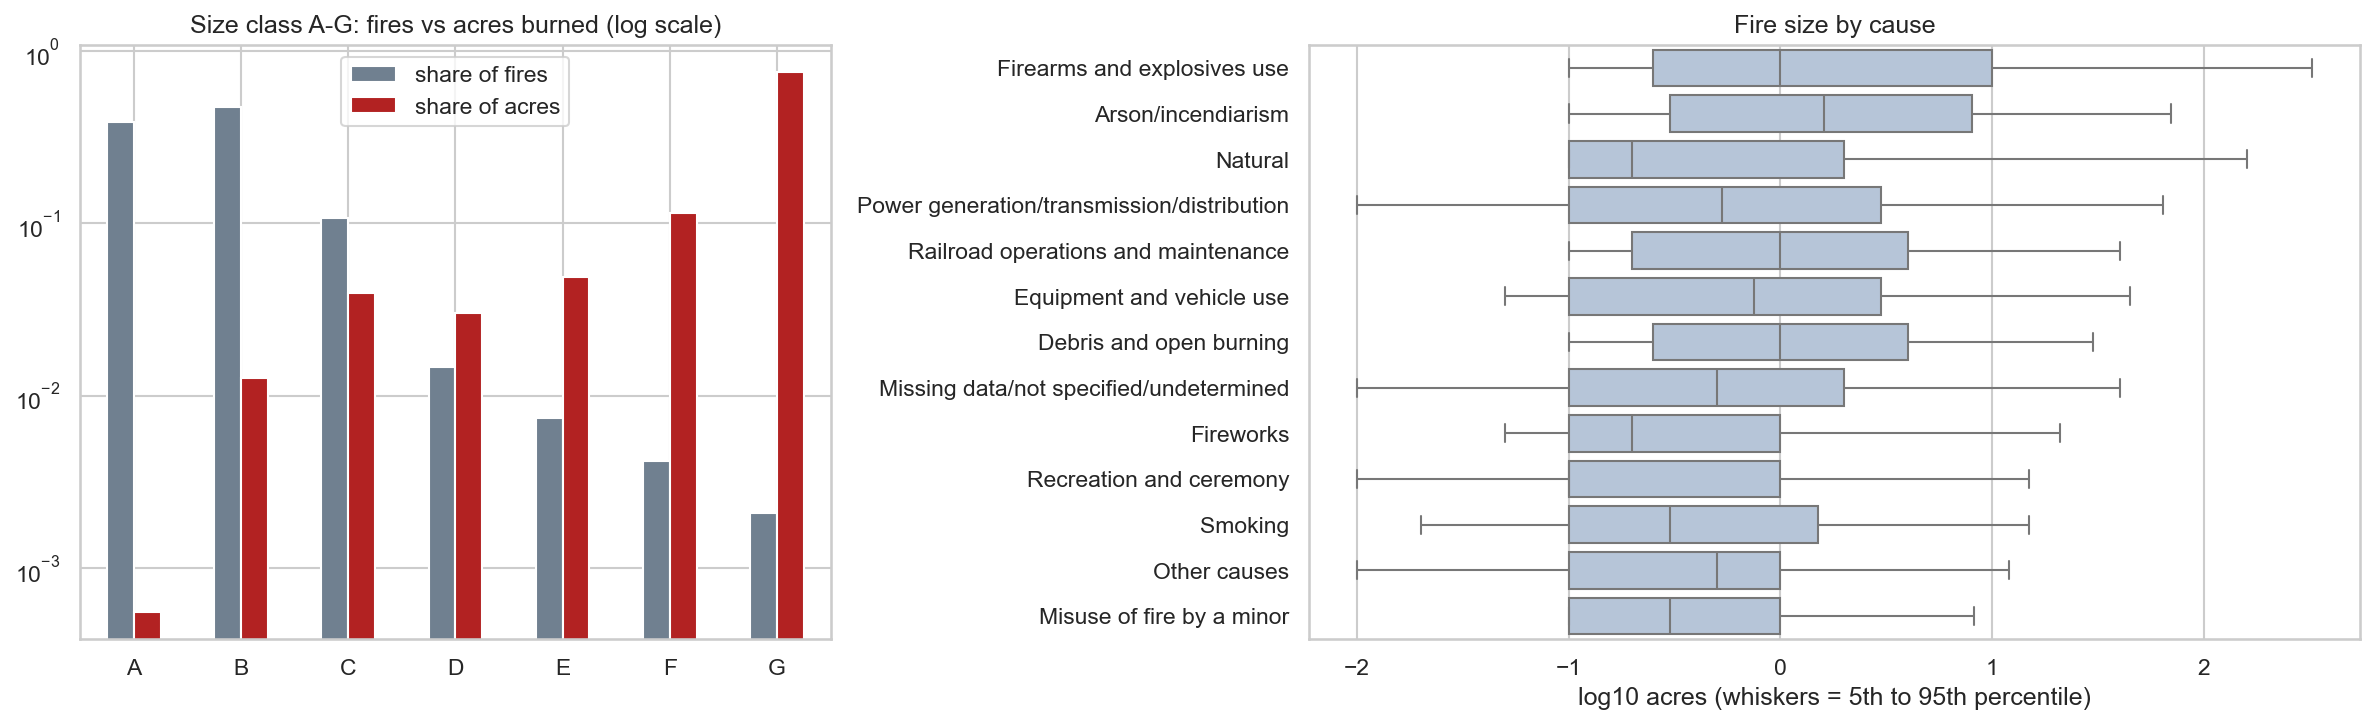
\includegraphics[width=\textwidth]{size_skew.png}
\caption{Left: share of fires vs.\ share of acres burned by size class A--G. Right: fire size by cause (log scale).}
\label{fig:size}
\end{figure*}

\subsection{Stations versus fires}
Figure~\ref{fig:stations} compares station and fire density. Stations are dense in the East and along the West Coast. They are sparse across the interior West, the northern Plains and south Texas, which still have many fires. That mismatch motivates both questions.
\begin{figure*}[t]
\centering
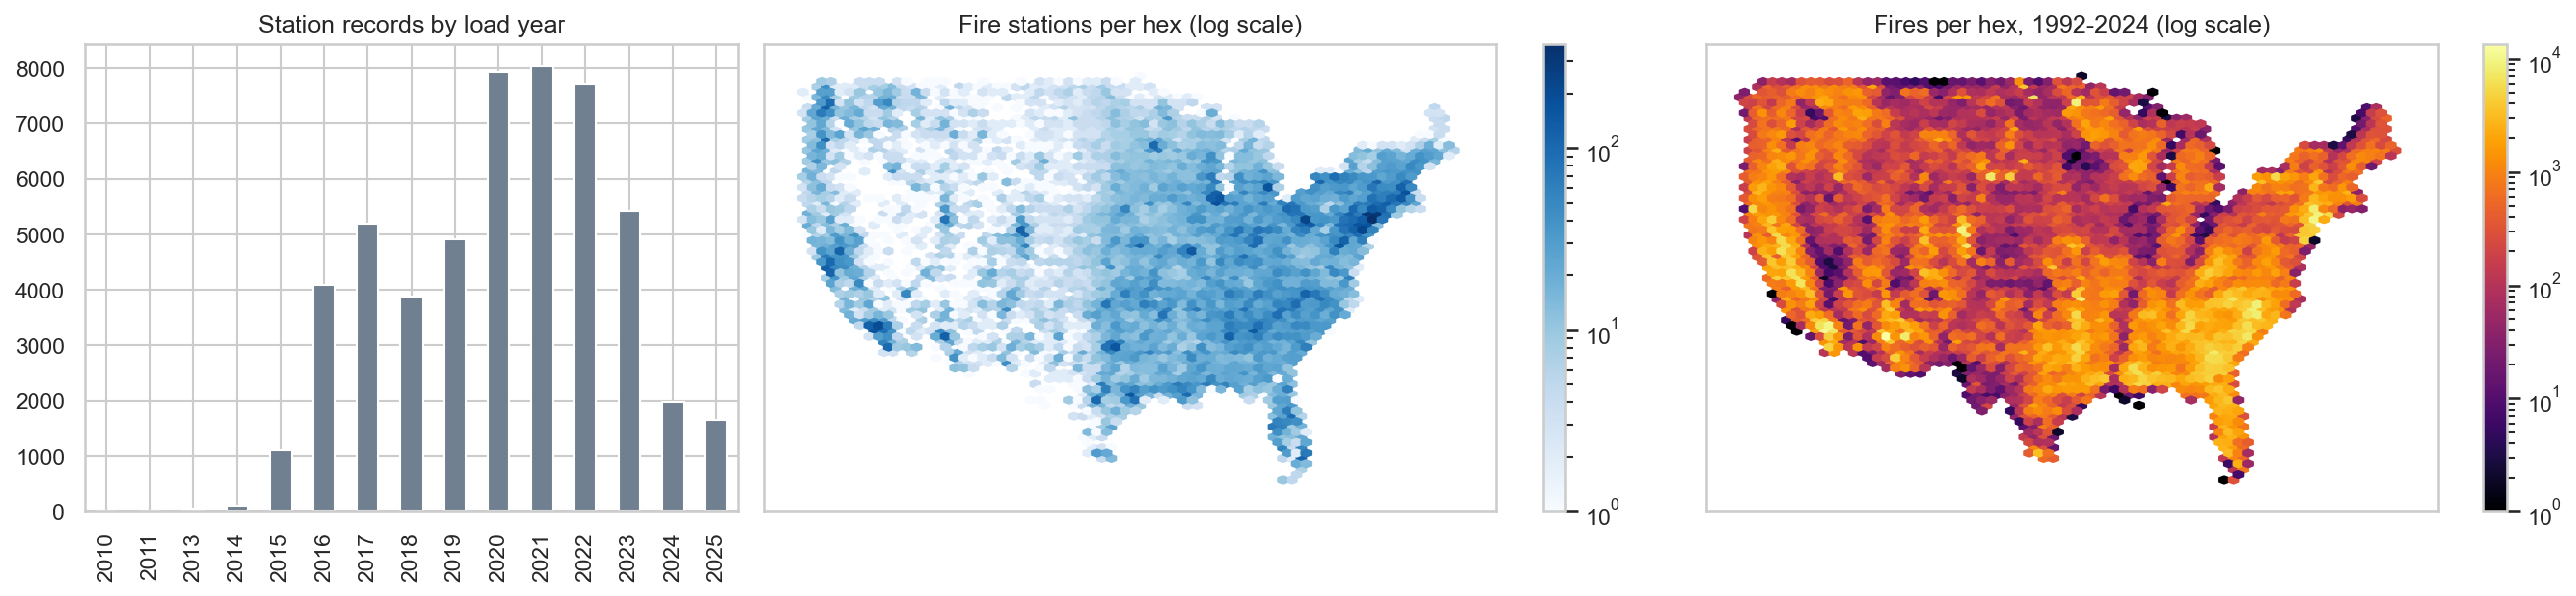
\includegraphics[width=\textwidth]{stations_vs_fires.png}
\caption{Left: station records by load year. Middle: fire stations per hex. Right: fires per hex, 1992--2024. Hex colour scales are logarithmic.}
\label{fig:stations}
\end{figure*}

\subsection{Distance from fires to stations}
For each fire we compute the great-circle (haversine) distance to the nearest station with a ball tree:
\begin{equation}
d = 2R\arcsin\!\sqrt{\sin^2\!\tfrac{\Delta\phi}{2}+\cos\phi_1\cos\phi_2\sin^2\!\tfrac{\Delta\lambda}{2}},
\end{equation}
where $\phi$ is latitude, $\lambda$ is longitude and $R = 6371$~km.
The median fire starts 4.2~km from a station. 90\% start within 13.9~km and 99\% within 39~km. Figure~\ref{fig:coverage} shows the key asymmetry. 58\% of fires start within 5~km of a station but account for only 13.6\% of acres burned. Within 10~km the figures are 84\% of fires and 31\% of acres, and within 20~km 94\% and 56\%. Most burned area comes from the small share of fires far from any station.

We also count the stations within 25~km of each fire (\code{STATIONS_25KM}), which says whether more help can follow the first engine. The median fire has 16, and 3.7\% of fires have none. Finally, we flag 4{,}219 fires on \emph{stacked} locations, exact coordinates shared by 200 or more fires. These are reporting offices and placeholders, so they are left out of the odds-ratio analysis below.
\begin{figure*}[t]
\centering
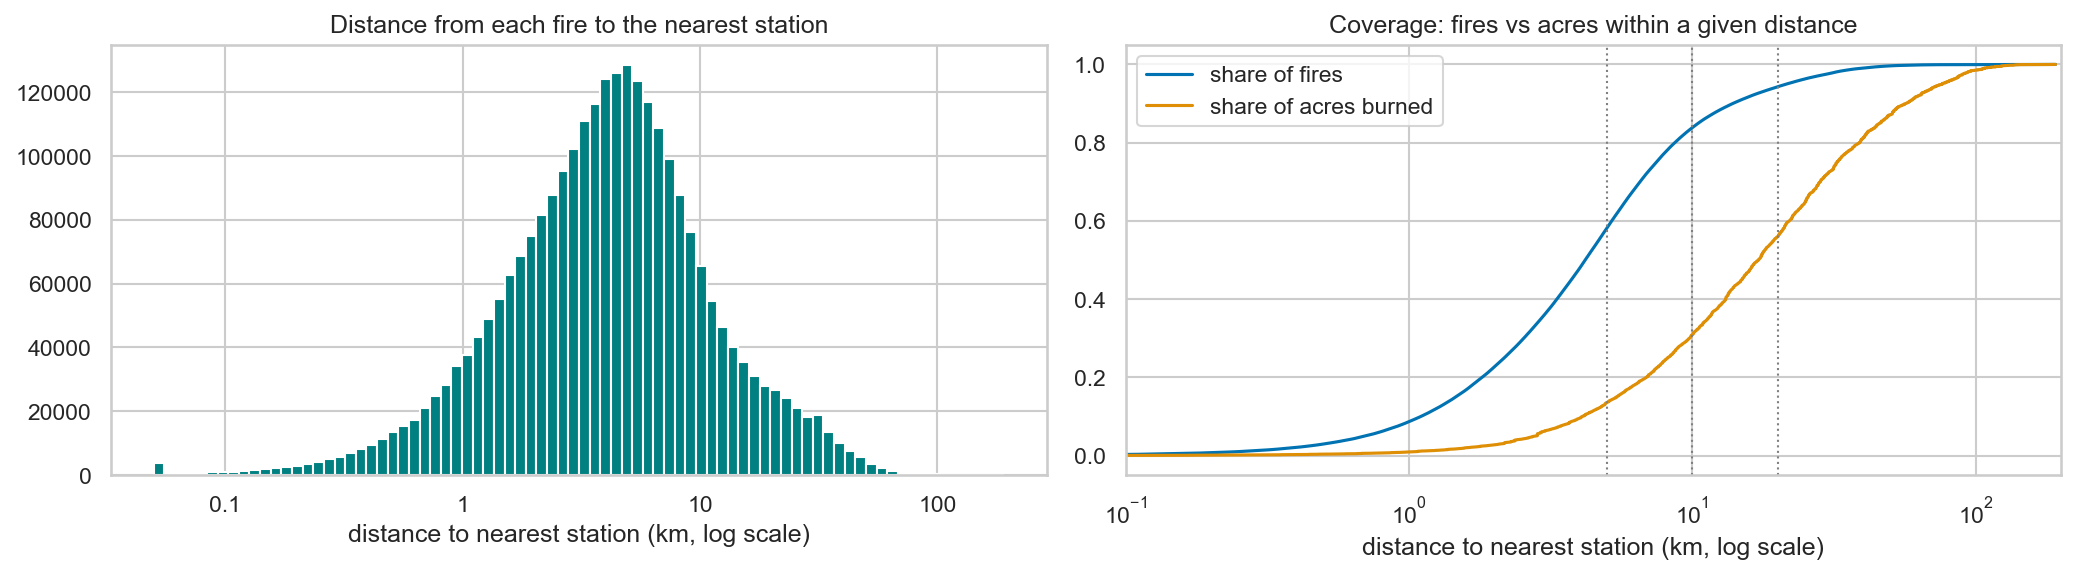
\includegraphics[width=\textwidth]{distance_coverage.png}
\caption{Left: distance to the nearest station (log scale). Right: cumulative share of fires and of acres burned within a given distance.}
\label{fig:coverage}
\end{figure*}

Far-from-station fires concentrate in the Great Basin, Montana, Wyoming, the northern Plains, south Texas and the Everglades (Figure~\ref{fig:owner}). The median distance ranges from 1.9~km on municipal land and 3.9~km on private land to 10.8~km on USFS land and 14.5~km on BLM land. Part of this is a data gap: federal land is protected by wildland crews that are mostly absent from the station layer. \code{DIST_KM} therefore means the distance to the nearest \emph{structural} station.
\begin{figure*}[t]
\centering
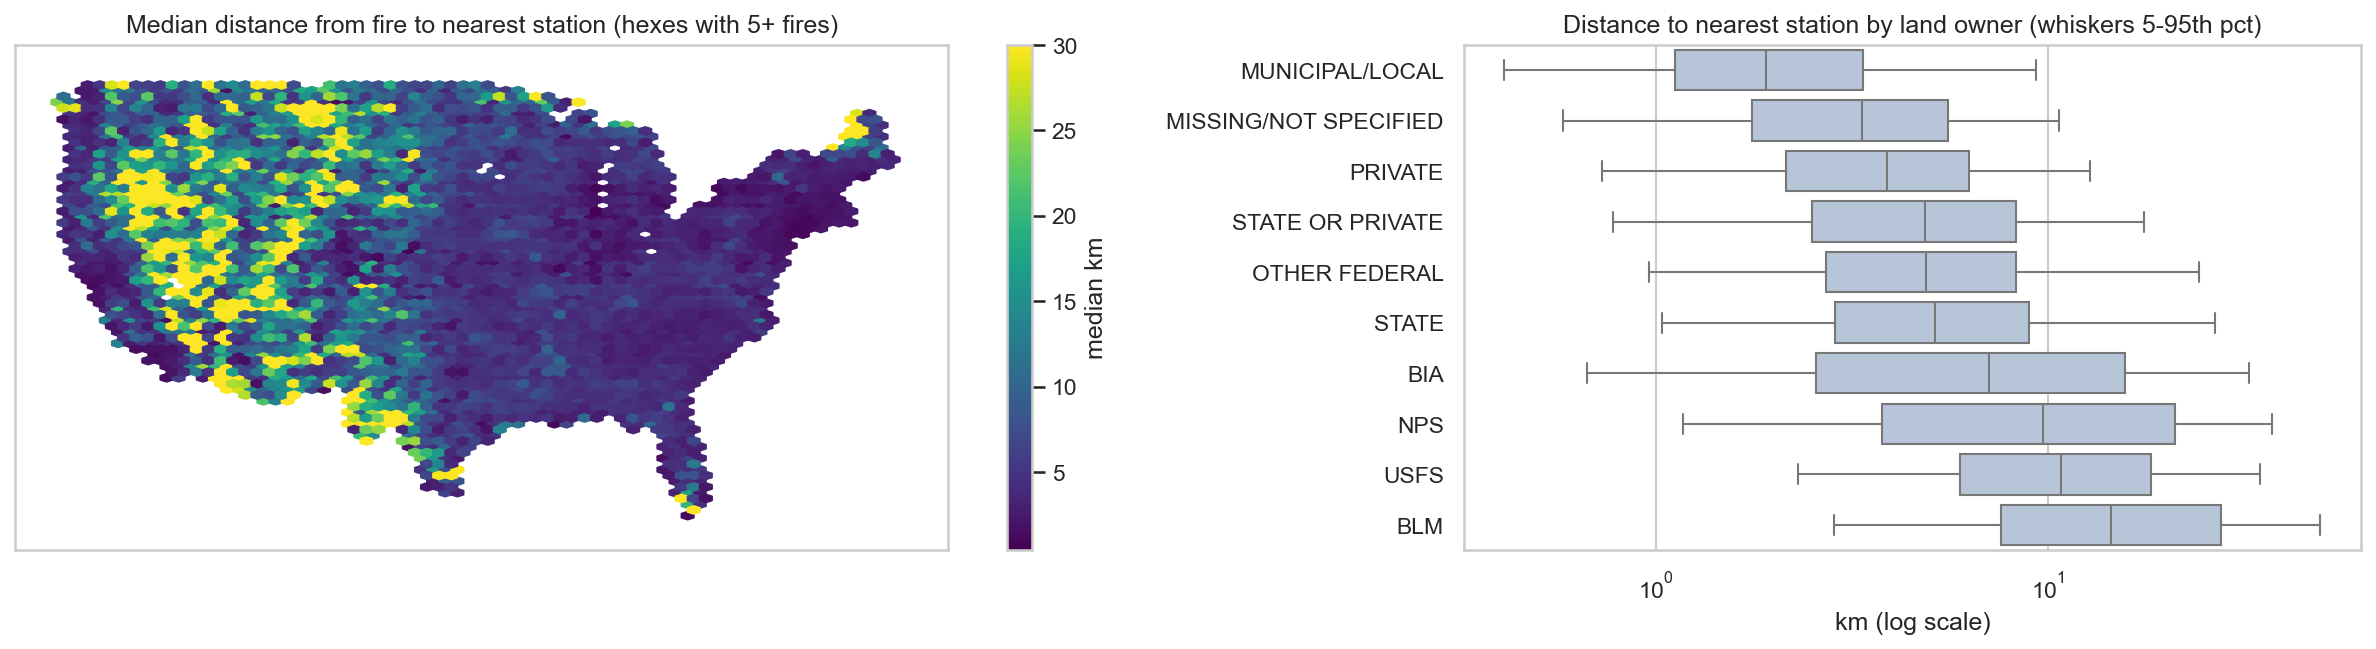
\includegraphics[width=\textwidth]{distance_map_owner.png}
\caption{Left: median fire-to-station distance per hex (hexes with 5+ fires). Right: distance by land owner (whiskers at the 5th and 95th percentiles).}
\label{fig:owner}
\end{figure*}

\subsection{RQ1: distance and fire outcomes}
\paragraph{Target.} $y=\mathbb{1}[\text{FIRE\_SIZE}\geq 100~\text{acres}]$ (size classes D--G). Positives are 2.91\% of the 1992--2018 training fires (63{,}207 of 2.17M) and 2.53\% of the 2019--2024 test fires (12{,}382 of 489k), about 1 positive per 34 negatives.

\paragraph{Gradient.} Table~\ref{tab:bands} and Figure~\ref{fig:bands} show that the share of large fires rises roughly 22-fold from the nearest to the farthest band. The mean containment time rises from 0.3 to 8.5 days. The lightning share rises from 3\% to 80\% across the same bands, so we check for confounding below.

\begin{table*}[t]
\centering\small
\caption{Fire outcomes by distance to the nearest station (all fires, 1992--2024).}
\label{tab:bands}
\begin{tabular}{@{}lrrrrr@{}}
\toprule
Distance (km) & Fires & Share large & Share of acres & Lightning share & Mean days to contain \\
\midrule
0--2   & 602{,}152 & 0.75\%  & 2.7\%  & 3.4\%  & 0.30 \\
2--5   & 946{,}940 & 1.74\%  & 10.9\% & 5.8\%  & 0.39 \\
5--10  & 682{,}126 & 3.41\%  & 17.3\% & 12.4\% & 0.61 \\
10--20 & 278{,}161 & 6.10\%  & 25.1\% & 37.0\% & 1.54 \\
20--40 & 127{,}730 & 8.03\%  & 25.2\% & 58.4\% & 2.89 \\
40+    & 24{,}274  & 16.89\% & 18.8\% & 79.9\% & 8.47 \\
\bottomrule
\end{tabular}
\end{table*}

\begin{figure*}[t]
\centering
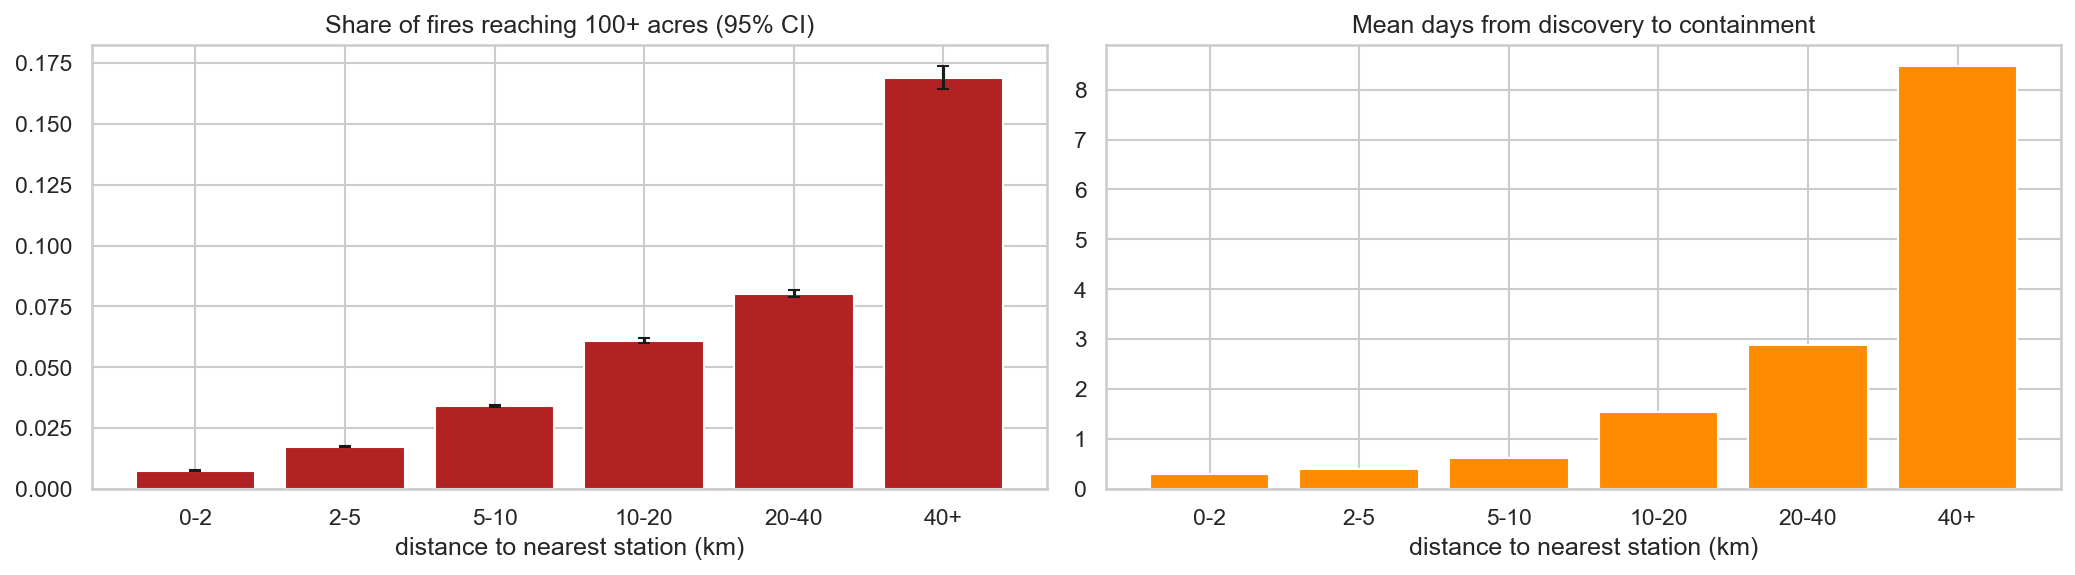
\includegraphics[width=\textwidth]{large_by_distance.png}
\caption{Left: share of fires reaching 100+ acres by distance band, with 95\% Wilson intervals. Right: mean days from discovery to containment (fires with a containment date).}
\label{fig:bands}
\end{figure*}

\paragraph{Confounding check.} If the gradient only reflected remote fires being lightning fires in the West, it would vanish within each region and cause class. It does not vanish (Figure~\ref{fig:strata}). Human-caused fires in the East rise from 0.75\% to 16.8\% large, and in the West from 0.67\% to 10.9\%. Lightning fires in the East rise from 1.2\% to 26\%, and in Alaska from 11\% to 49\%. The flattest line is western lightning fires (1.9\% to 11.5\%), which burn mostly on federal land covered by wildland crews that are not in the station layer. The curves for 1992--2014 and 2015--2024 nearly coincide, so the station snapshot's timing does not drive the result.

\begin{figure*}[t]
\centering
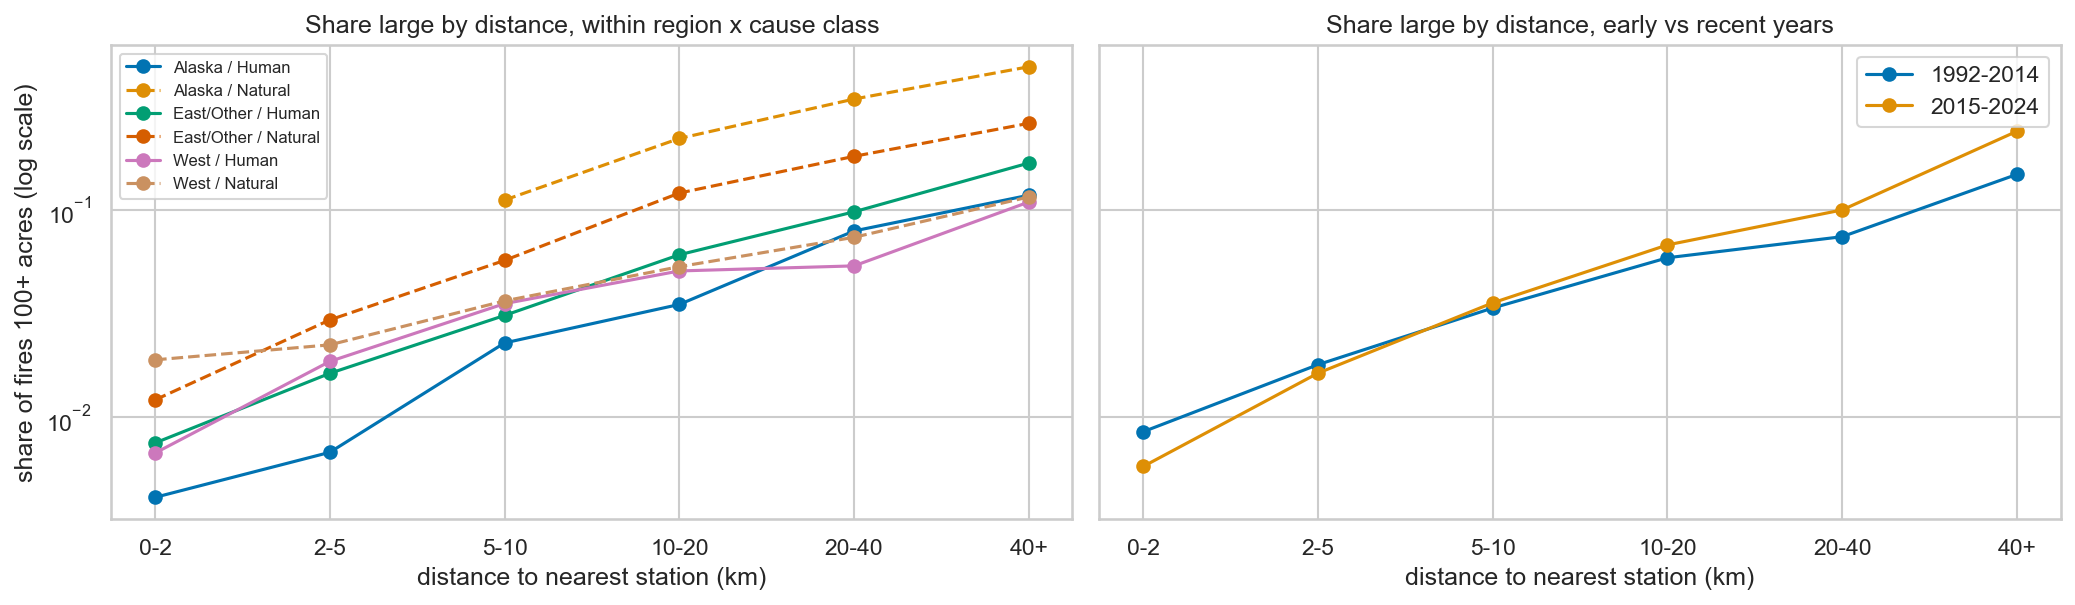
\includegraphics[width=\textwidth]{large_by_distance_strata.png}
\caption{Share of large fires by distance (log scale). Left: within region $\times$ cause class (strata with 200+ fires). Right: 1992--2014 versus 2015--2024.}
\label{fig:strata}
\end{figure*}

\paragraph{Size cutoffs and under-reporting.} If small remote fires simply went unreported, the share of large fires would rise with distance even if distance did nothing. Two checks argue against this (Figure~\ref{fig:cutoffs}). First, the rise is steeper for stricter cutoffs. From the nearest to the farthest of 20 equal-size distance bins, fires of 10+ acres go from 4.6\% to 17.4\% (3.8$\times$), 100+ acres from 0.64\% to 8.4\% (13$\times$), and 1{,}000+ acres from 0.10\% to 3.1\% (33$\times$). Second, tiny class~A fires do not vanish far from stations: their share is 55\% in the nearest bin, falls to 29\% around 6~km, and climbs back to 52\% in the farthest bin.

\begin{figure*}[t]
\centering
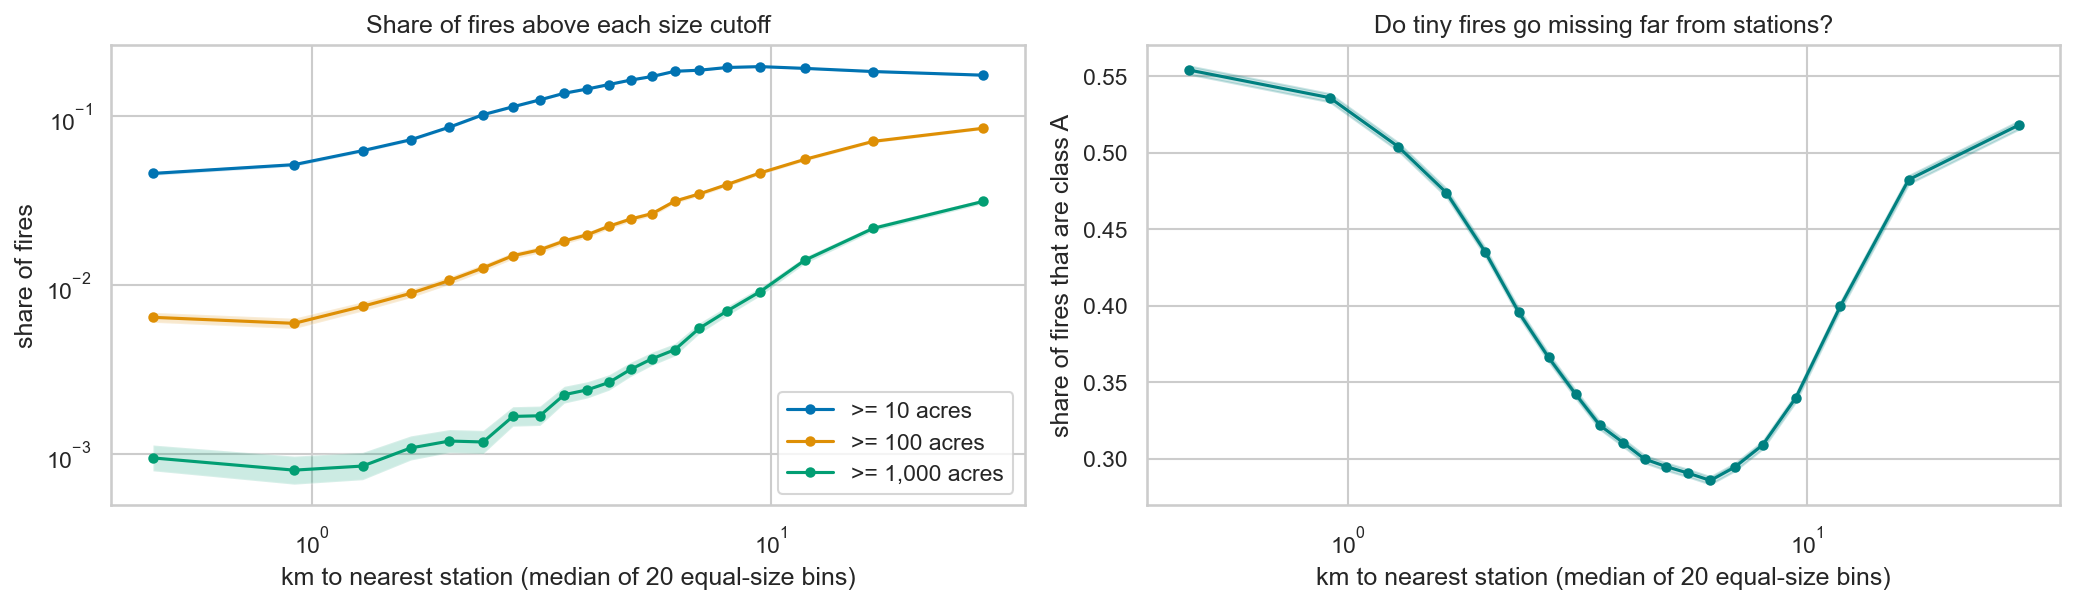
\includegraphics[width=\textwidth]{size_cutoffs.png}
\caption{Left: share of fires above 10, 100 and 1{,}000 acres by distance (20 equal-size bins, 95\% Wilson intervals, log scales). Right: share of tiny class~A fires by distance.}
\label{fig:cutoffs}
\end{figure*}

\paragraph{Odds ratios.} To put one number on the effect, we fit a logistic regression of the target on $\log_2(d+1)$, with $d$ in km, and controls $\mathbf{c}$:
\begin{equation}
\operatorname{logit} P(y=1) = \beta_0 + \beta_1 \log_2(d+1) + \boldsymbol{\gamma}^\top\mathbf{c}.
\end{equation}
$e^{\beta_1}$ is the odds multiplier for each doubling of $(d+1)$. We use lower-48 fires without stacked locations (2.60M fires) and a fixed sample of 300k per fit. The 95\% Wald intervals assume independent fires; neighbouring fires are correlated, so the true intervals are wider. We read them as effect sizes, not significance tests.

Table~\ref{tab:or} shows the result. Each doubling multiplies the odds of a large fire by 1.90 unadjusted and by \textbf{1.80 after adjusting for state, land owner, month and year}. Adding cause barely changes it (1.79), and 89\% of the raw excess odds survives adjustment. The effect grows with the cutoff (1.55, 1.80, 2.07 for 10, 100 and 1{,}000 acres), as expected if distance matters most for fires that escape initial attack. Inside each of the 17 region, owner and cause groups the odds ratio ranges from 1.26 to 2.77, and every interval is above 1 (Figure~\ref{fig:orgroup}). It is weakest on federal land (BIA 1.26, BLM 1.33, USFS 1.35) and for lightning fires (1.54), where wildland crews missing from the station layer do the initial attack. It is strongest in the North/East (2.77) and Southeast (2.19), where municipal and county stations are the first responders.

\begin{table}[tb]
\centering\footnotesize
\caption{Odds ratio per doubling of distance (target $\geq$100 acres unless noted). ``Adjusted'' controls for state, land owner, month and year.}
\label{tab:or}
\begin{tabularx}{\columnwidth}{@{}Xcc@{}}
\toprule
Estimate & OR & 95\% CI \\
\midrule
Unadjusted & 1.90 & 1.86--1.93 \\
Adjusted & \textbf{1.80} & 1.76--1.84 \\
Adjusted + cause class & 1.79 & 1.74--1.83 \\
\midrule
Adjusted, target $\geq$10 acres & 1.55 & 1.53--1.57 \\
Adjusted, target $\geq$1{,}000 acres & 2.07 & 1.97--2.18 \\
\midrule
Adjusted, 1992--2018 & 1.77 & 1.72--1.81 \\
Adjusted, 2019--2024 & 2.03 & 1.98--2.08 \\
\midrule
Adjusted, 25\% of stations removed & 1.70 & 1.66--1.74 \\
Adjusted, 50\% of stations removed & 1.61 & 1.57--1.65 \\
Adjusted, 75\% of stations removed & 1.46 & 1.43--1.50 \\
\bottomrule
\end{tabularx}
\end{table}

\begin{figure}[tb]
\centering
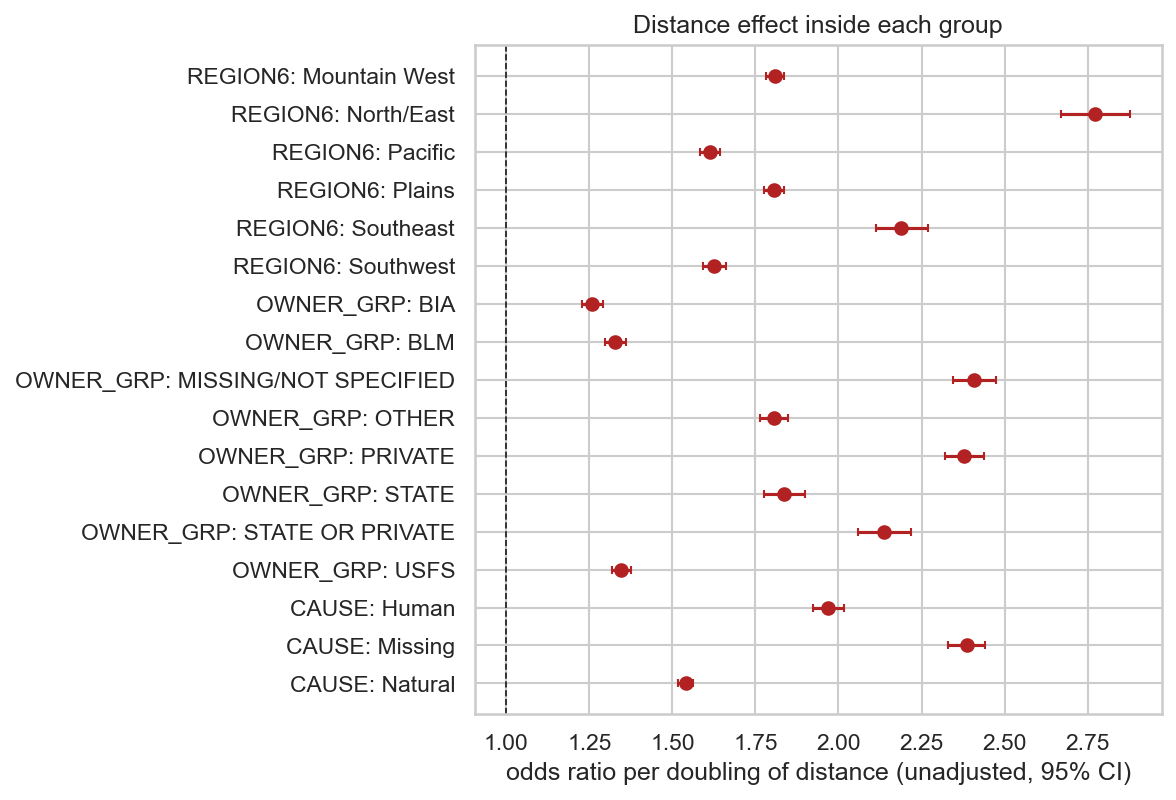
\includegraphics[width=\columnwidth]{or_by_group.png}
\caption{Unadjusted odds ratio per doubling of distance inside each region, land-owner group and cause class (95\% CI). All 17 are above 1.}
\label{fig:orgroup}
\end{figure}

\paragraph{Stability over time.} The yearly odds ratio is above 1 in all 33 years, ranging from 1.53 to 2.30 (Figure~\ref{fig:oryear}). It is larger in recent years: 1.77 for 1992--2018 against 2.03 for 2019--2024 (adjusted). Two explanations fit, and the data cannot separate them. The station layer was mostly loaded in 2015--2023, so it describes recent years better. The 2020--21 reporting changes also altered which fires are recorded. For Milestone~2 this means the test years carry a somewhat stronger distance signal than the training years.

\begin{figure}[tb]
\centering
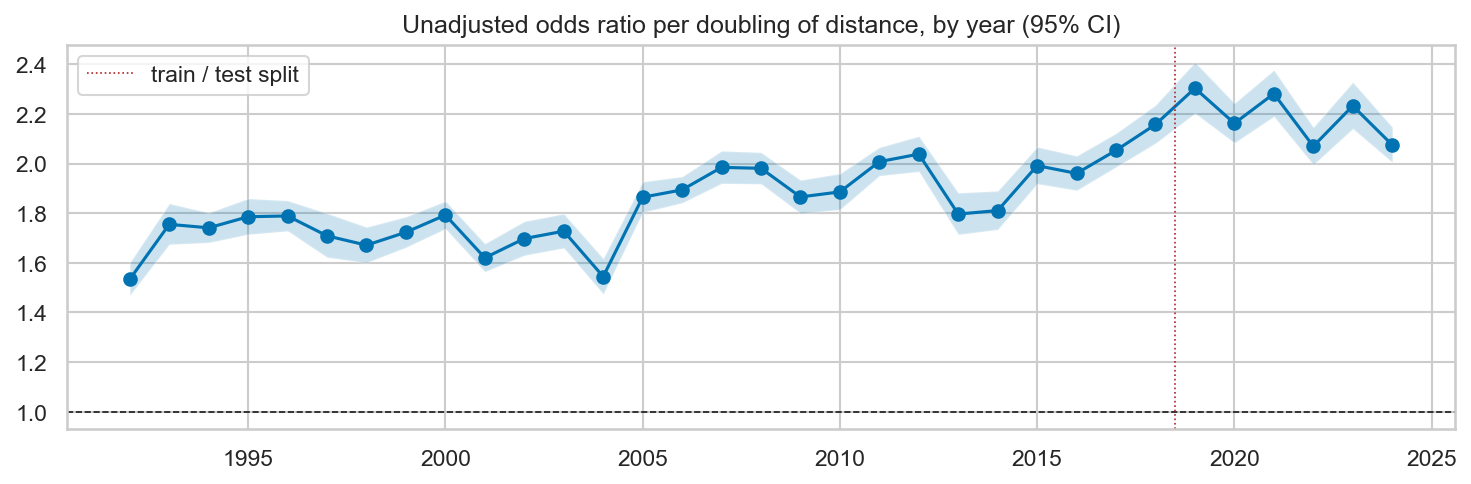
\includegraphics[width=\columnwidth]{or_by_year.png}
\caption{Unadjusted odds ratio per doubling of distance by year (95\% CI). The dotted line marks the train/test split.}
\label{fig:oryear}
\end{figure}

\paragraph{Sensitivity to the station list.} The station layer is incomplete, and a missing station makes nearby fires look farther from help. We delete 25\%, 50\% and 75\% of stations at random and refit (Table~\ref{tab:or}). The adjusted odds ratio falls from 1.80 to 1.70, 1.61 and 1.46 but stays above 1. Random errors in distance dilute the estimate toward 1. So if stations are missing at random, our estimate is more likely too small than too large. Stations missing systematically, such as wildland bases on federal land, could bias it either way.

\paragraph{Baseline viability.} We train on 1992--2018 and test on 2019--2024 (Table~\ref{tab:baseline}, Figure~\ref{fig:pr}). The base LightGBM already sees latitude, longitude, state, day of year, cause class and land owner. Adding distance still improves PR-AUC by 29\% (relative). Distance to the nearest of 52k points cannot be rebuilt from raw coordinates, so the station join adds information. Absolute PR-AUC is modest because final size also depends on weather and fuel, which are not in the data.

Cause is only known after an investigation, so a model used at discovery time cannot see it. Without cause, the base model reaches 0.129 PR-AUC, slightly \emph{higher} than with cause. Distance still lifts it to 0.147, and adding the number of stations within 25~km lifts it to \textbf{0.163}, the best of all variants. The station signal therefore does not depend on cause, and a discovery-time model is a realistic main model for Milestone~2.

\begin{table}[tb]
\centering\small
\caption{Untuned baselines on the 2019--2024 hold-out (target: $\geq$100 acres).}
\label{tab:baseline}
\begin{tabularx}{\columnwidth}{@{}Xcc@{}}
\toprule
Model & ROC-AUC & PR-AUC \\
\midrule
No skill (prevalence) & 0.500 & 0.025 \\
Logistic regression, $\log(1+d)$ only, balanced weights & 0.756 & 0.097 \\
LightGBM, location + season + cause + owner & 0.813 & 0.119 \\
LightGBM, same + distance & 0.840 & 0.153 \\
LightGBM, same + distance + stations within 25~km & 0.845 & 0.160 \\
\midrule
LightGBM, location + season + owner (no cause) & 0.817 & 0.129 \\
LightGBM, no cause + distance & 0.842 & 0.147 \\
LightGBM, no cause + distance + stations within 25~km & \textbf{0.848} & \textbf{0.163} \\
\bottomrule
\end{tabularx}
\end{table}

\begin{figure}[tb]
\centering
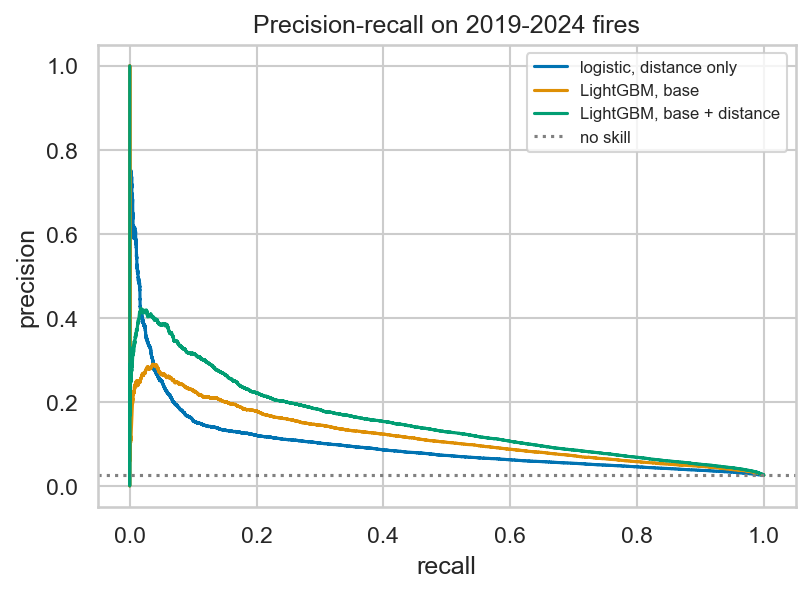
\includegraphics[width=\columnwidth]{pr_curves.png}
\caption{Precision--recall curves on 2019--2024 fires.}
\label{fig:pr}
\end{figure}

\subsection{RQ2: under-served areas}
A single fire is too noisy to characterise an area, so we cluster \emph{places}. We divide the lower 48 states into roughly 25~km $\times$ 25~km cells and keep cells with at least 30 fires over 33 years (9{,}087 cells). A cell is \emph{under-served} if its median fire is 10~km or more from the nearest station. That leaves 2{,}271 cells, which hold 11.5\% of lower-48 fires but \textbf{41.8\% of the acres burned}.

\paragraph{Features.} Each cell is described by eleven features. They are the log fire rate, the share of large fires, the median and 90th-percentile log size, the summer share, the circular mean of the discovery day (sine and cosine), the weekend share, the log median distance, and the federal and private land shares. \textbf{Cause is held out} and used only to validate the clusters. The three size features are correlated (0.77--0.84), the summer share mirrors the season pair ($\approx -0.88$), and the federal and private shares are near opposites ($-0.81$). The held-out lightning share correlates with the summer share (0.77) and the federal share (0.60).

\paragraph{Cluster tendency and $k$.} The Hopkins statistic \cite{hopkins1954} is 0.82, stable across 10 draws and well above the 0.5 expected for uniform data. Silhouette \cite{rousseeuw1987} peaks at $k=2$ (0.29) and Davies--Bouldin \cite{davies1979} is lowest at $k=3$ (1.47), with no sharp elbow (Figure~\ref{fig:ksel}). $k=2$ only separates western federal land from everything else, so we take $k=4$ as a preliminary, interpretable choice. Its silhouette of 0.19 indicates overlapping groups, which Milestone 3 addresses.

\begin{figure*}[t]
\centering
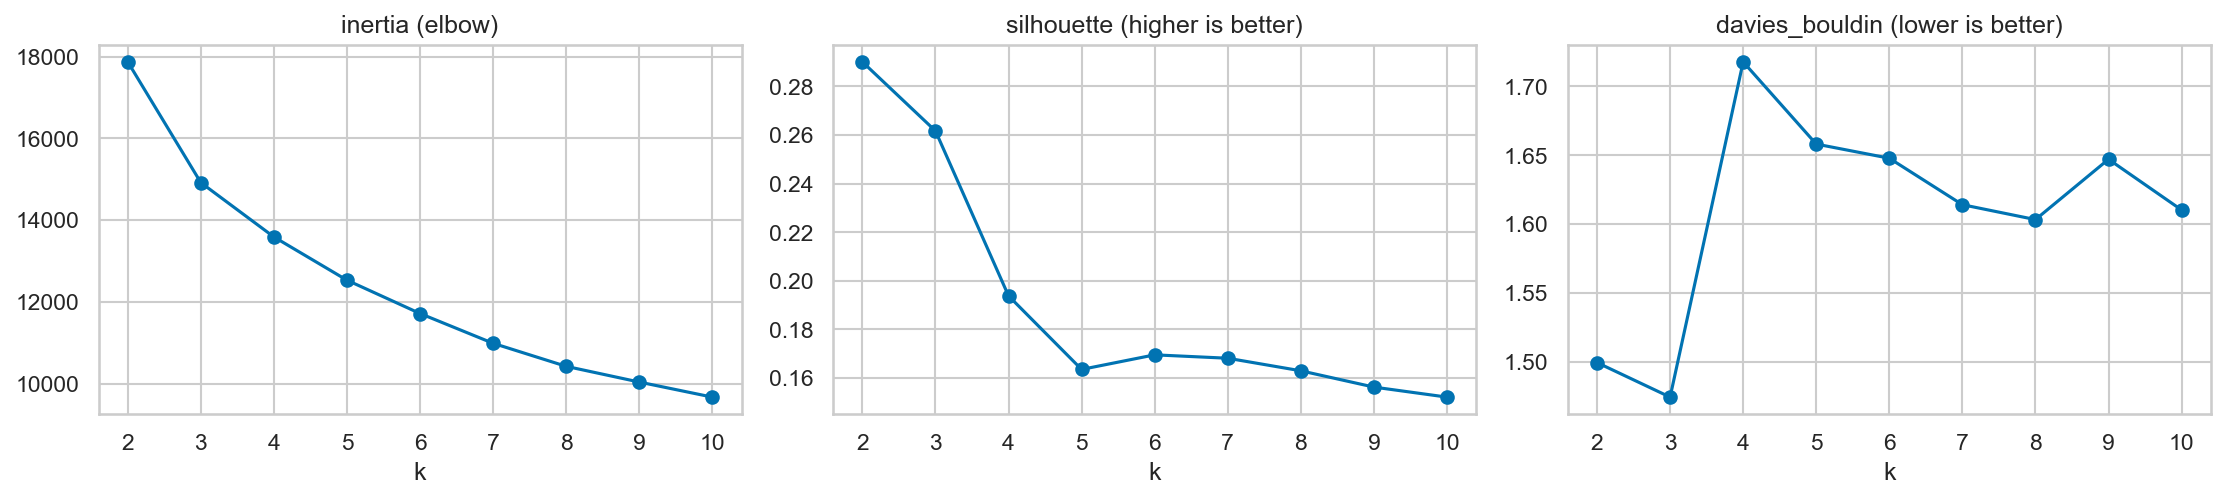
\includegraphics[width=\textwidth]{cluster_selection.png}
\caption{K-Means model selection on under-served cells: inertia, silhouette and Davies--Bouldin for $k=2,\dots,10$.}
\label{fig:ksel}
\end{figure*}

\begin{figure*}[t]
\centering
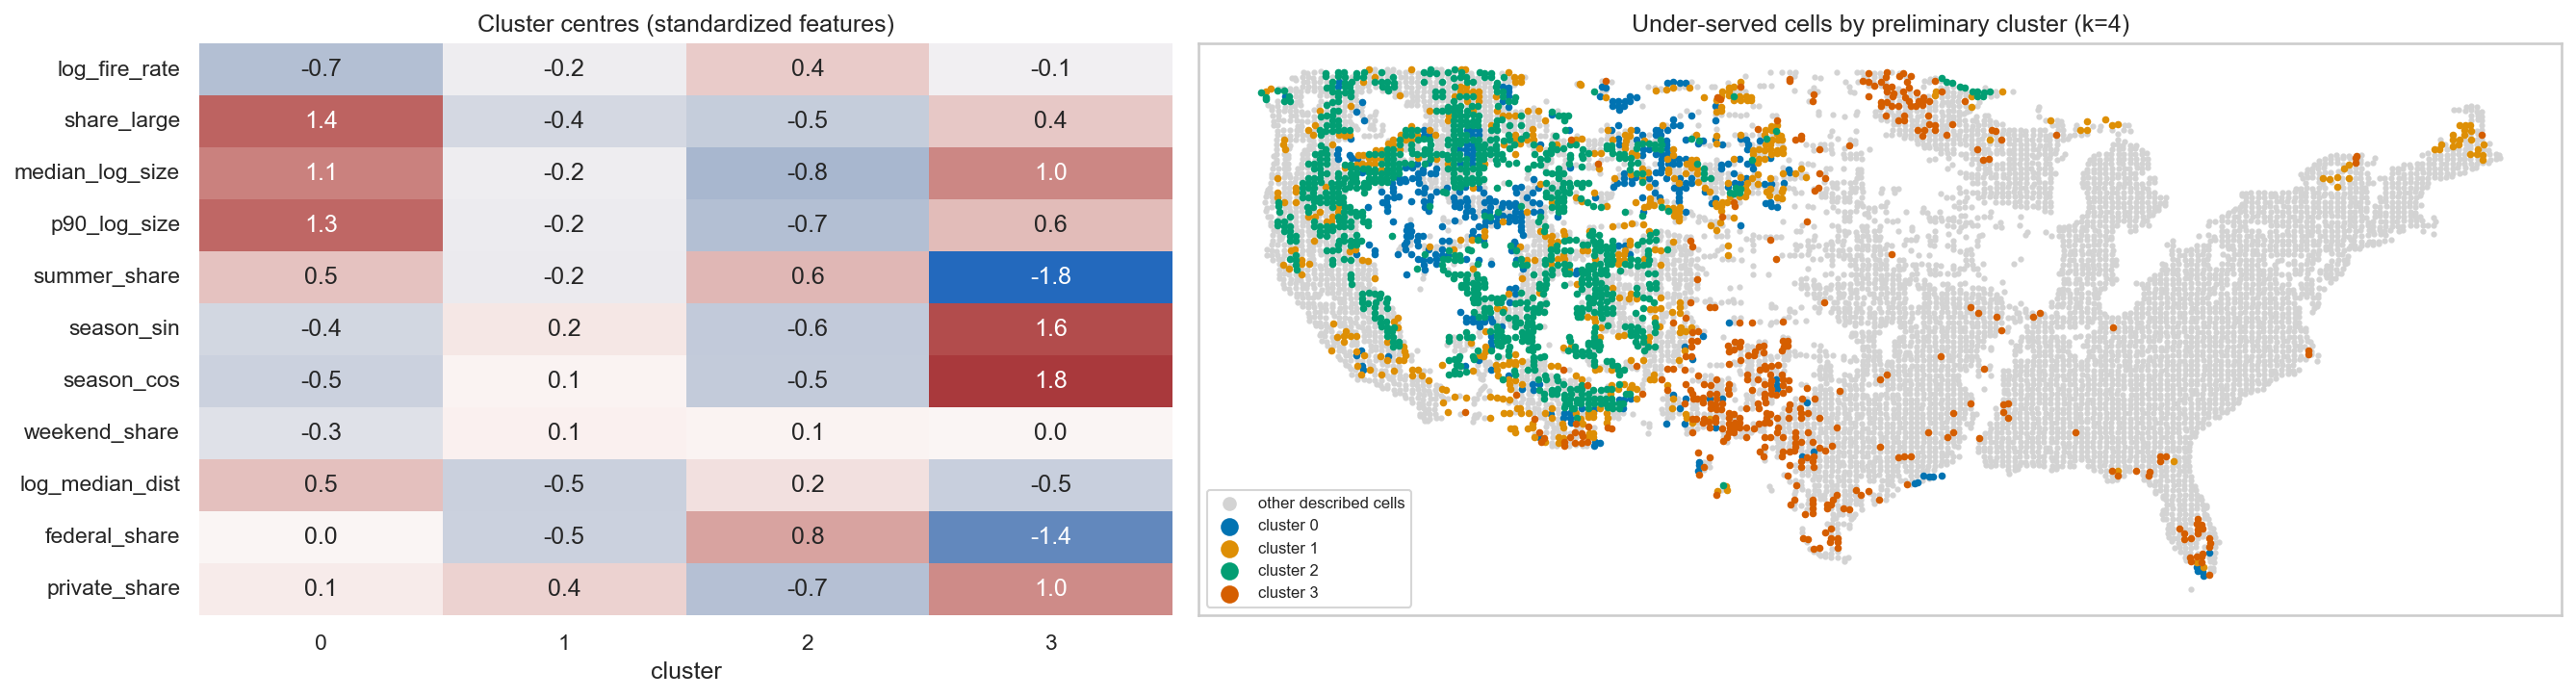
\includegraphics[width=\textwidth]{cluster_profile_map.png}
\caption{Preliminary $k=4$ clustering. Left: standardised cluster centres. Right: under-served cells coloured by cluster (grey: other cells with 30+ fires).}
\label{fig:clusters}
\end{figure*}

\begin{table*}[t]
\centering\small
\caption{Preliminary types of under-served area. The lightning share was \emph{not} used for clustering.}
\label{tab:clusters}
\begin{tabularx}{\textwidth}{@{}lrXrX@{}}
\toprule
Type & Cells & Fire behaviour & Lightning & Where \\
\midrule
0 Remote large-fire wildlands & 393 & fewest fires; 24\% become large; summer; median 24~km from a station & 62\% & Great Basin, MT, WY \\
1 Mixed rural fringe & 534 & near average; slightly more private land & 36\% & edges of the West, upper Midwest, N.\ New England \\
2 Busy federal forests & 968 & most fires, but tiny (median $\approx$0.1~acre); summer; 88\% federal & 70\% & Rockies, Sierra Nevada, AZ/NM \\
3 Spring private-land fires & 376 & spring peak (34\% summer); 45\% private; 14\% large & 15\% & OK/TX, Florida, N.\ Minnesota \\
\bottomrule
\end{tabularx}
\end{table*}

The held-out lightning share ranges from 15\% to 70\% across clusters (Table~\ref{tab:clusters}), so the clusters capture real differences in fire regime. Cluster~2 shows the data gap: it is far from structural stations, yet its fires stay tiny because national forests have their own wildland crews.

\paragraph{Are the clusters real?} Refitting on 30 bootstrap resamples gives an adjusted Rand index of 0.88 $\pm$ 0.15 with the main labels. Most refits reproduce the four groups, but some split them differently, which fits the low silhouette. Dropping one feature group at a time shows what drives the clusters. Removing season (ARI 0.34), the size features (0.35) or land owner (0.42) changes them a lot, while removing distance (0.85), fire rate (0.89) or weekend share (0.96) changes them little. Distance matters less here because every cell is already under-served. A Gaussian mixture agrees only moderately with K-Means (ARI 0.45), and its BIC prefers $k=6$. The land-owner and region mix of each cluster, which were not inputs, match the cluster names (Figure~\ref{fig:heldout}). Cluster~0 is 65\% Mountain West and 33\% BLM land, and cluster~2 is 52\% Forest Service land. Cluster~3 has almost no western fires: it spans the Plains (33\%), Southeast (27\%) and North/East (26\%), mostly on private or unlisted land (69\%).

\begin{figure*}[t]
\centering
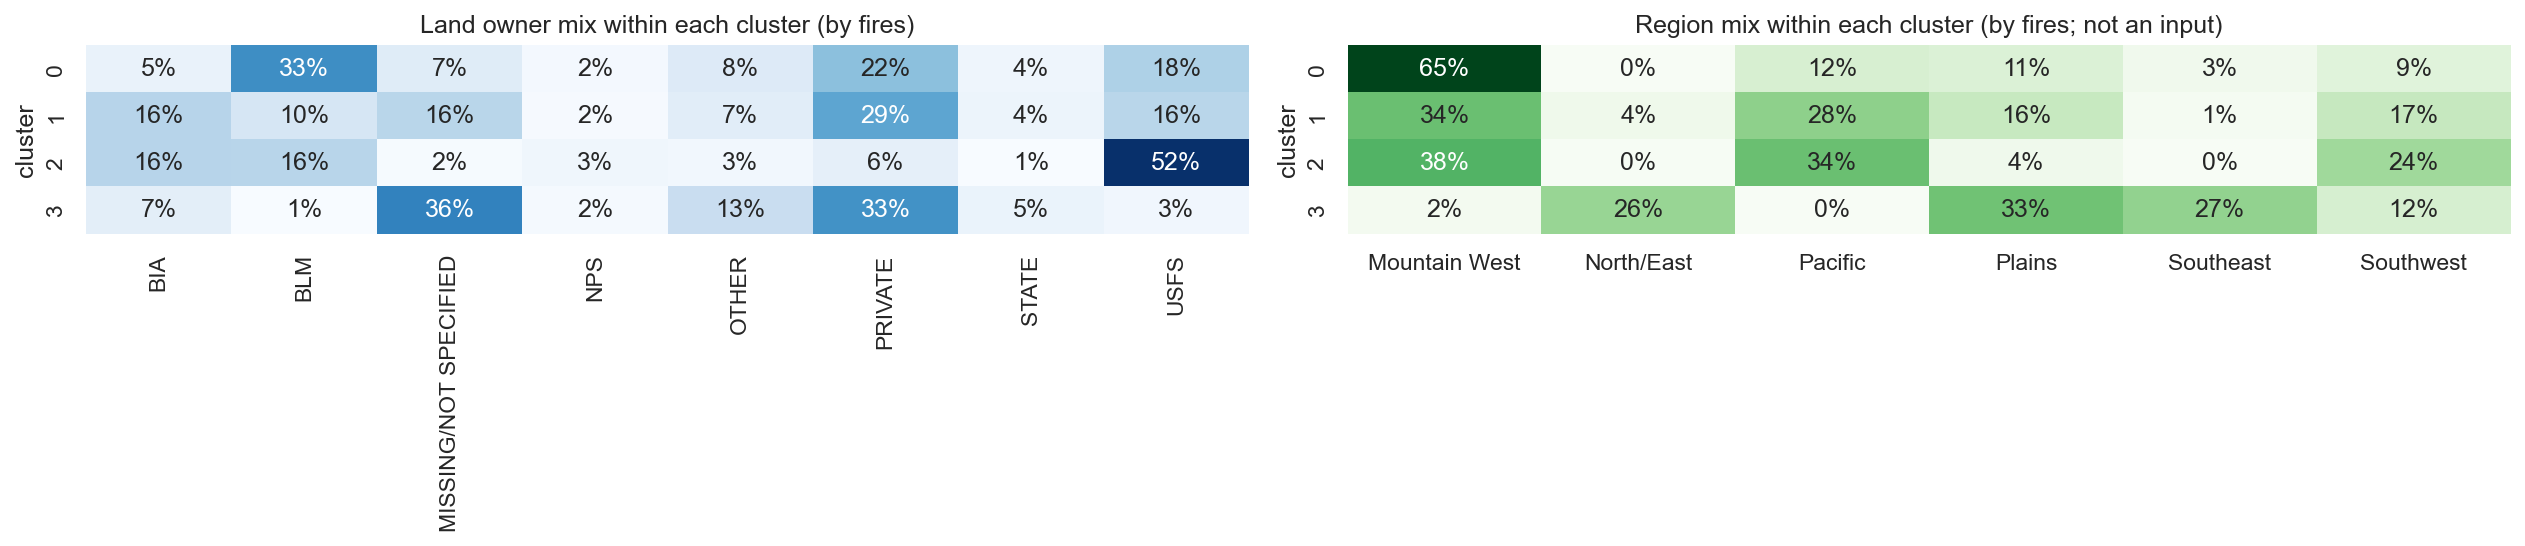
\includegraphics[width=\textwidth]{cluster_heldout.png}
\caption{Land-owner mix (left) and region mix (right) within each cluster, weighted by fires. Neither the full owner breakdown nor region was used for clustering.}
\label{fig:heldout}
\end{figure*}

\paragraph{From types to help.} To make the step from a cluster profile to a recommendation explicit, each type of help gets a scoring rule. The score is a weighted sum of the cluster's standardised centre $\mathbf{z}$, $s=\sum_f w_f z_f / \sum_f |w_f|$, and a cluster gets a suggestion when $s \geq 0.5$. For example, remote detection weights distance, share large and 90th-percentile size equally, and prevention weights fire rate and private land up and summer share down. The rules reproduce the recommendations above (Table~\ref{tab:help}). That is reassuring but not independent, since we wrote both.

\begin{table}[tb]
\centering\footnotesize
\caption{Suggested help per cluster from the scoring rules (score in brackets; threshold 0.5).}
\label{tab:help}
\begin{tabularx}{\columnwidth}{@{}>{\raggedright\arraybackslash}p{2.3cm}X@{}}
\toprule
Type & Suggested help \\
\midrule
0 Remote large-fire wildlands & remote detection and fast initial attack (1.08); extended-attack and surge capacity (1.08) \\
1 Mixed rural fringe & maintain current coverage \\
2 Busy federal forests & maintain current coverage \\
3 Spring private-land fires & new or volunteer station (0.78); prevention and outreach (0.58) \\
\bottomrule
\end{tabularx}
\end{table}

\paragraph{Circularity.} The clusters and the help rules both rely partly on fire size, which is the RQ1 target. Calling an area under-served partly because its fires are big is therefore circular. Milestone~3 reruns the clustering without the size features to see which types survive.

\paragraph{Would more stations close the gaps?} We place new stations greedily to cover as many uncovered 1992--2018 large fires as possible within 10~km, then score the 2019--2024 large fires the placement never saw (Figure~\ref{fig:budget}). With 200 new stations, coverage of large fires rises only from 57.4\% to 61.3\%, and coverage of their acres from 31.3\% to 37.9\%. The first 100 sites fall mainly in clusters 0 (32) and 3 (25). More stations alone do not close the gap, so the typology, which matches each area type to the help it needs, is the more useful output.

\begin{figure}[tb]
\centering
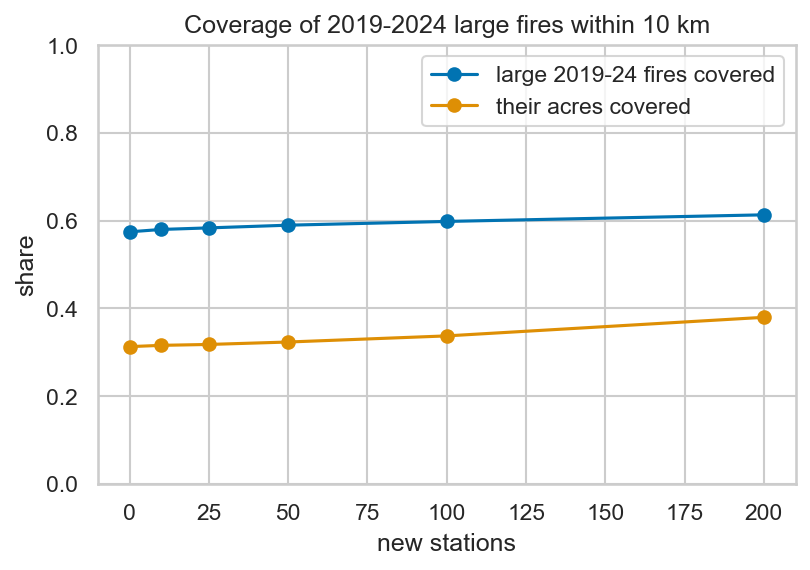
\includegraphics[width=\columnwidth]{coverage_budget.png}
\caption{Coverage of 2019--2024 large fires (and their acres) within 10~km as greedily placed stations are added.}
\label{fig:budget}
\end{figure}

%=====================================================================
\section{Methods}
%=====================================================================
\subsection{Supervised pipeline (RQ1, Milestone 2)}
\paragraph{Features.} The main predictor is $d_1$, the distance to the nearest station. We add engineered station features: the number of stations within 25~km (already computed), and $d_2$ and $d_3$ (second and third nearest stations). Controls are latitude, longitude, state, day of year encoded cyclically, weekday, land owner, and discovery hour with a missing-value flag. Cause class is only known after an investigation. It is a control in the explanatory model, and the predictive model is reported both with and without it. The cyclical encoding is
\begin{align}
\text{doy}_{\sin}&=\sin\!\left(2\pi\,\text{doy}/365.25\right),\\
\text{doy}_{\cos}&=\cos\!\left(2\pi\,\text{doy}/365.25\right).
\end{align}

\paragraph{Leakage prevention.} We exclude \code{FIRE_SIZE_CLASS} and all containment fields, because they are the outcome. We exclude \code{MTBS_ID} and the ICS-209 join IDs, because they exist only for large fires. We also exclude \code{FIRE_NAME}, and \code{SOURCE_SYSTEM_TYPE}, which encodes the year. Validation follows the spec's temporal rule: train on 1992--2018 and test on 2019--2024. Hyperparameters are tuned with time-blocked folds inside the training years, never with random $k$-fold. Because neighbouring fires are correlated, we add a spatial check that holds out whole regions. Fires on stacked office locations are dropped.

\paragraph{Imbalance.} We compare class-weighted losses with random undersampling of small fires. For the weighted logistic regression,
\begin{multline}
\mathcal{L}(\mathbf{w}) = -\sum_{i} \alpha_{y_i}\big[y_i\log\sigma(\mathbf{w}^\top\mathbf{x}_i)\\
+ (1-y_i)\log(1-\sigma(\mathbf{w}^\top\mathbf{x}_i))\big] + \lambda\lVert\mathbf{w}\rVert_2^2,
\end{multline}
where $\alpha_c = N/(2N_c)$ and $N_c$ is the number of fires in class $c$. The decision threshold is chosen on validation folds to maximise $F_1$.

\paragraph{Models.} We compare three families: L2 logistic regression (which also gives the odds ratio), random forest, and gradient-boosted trees (LightGBM \cite{ke2017}, plus XGBoost). Each is trained with and without the station features, and tuned with Optuna (Bayesian optimisation) during the optimisation phase.

\paragraph{Metrics.} PR-AUC is the primary metric, because it is more informative than ROC-AUC at 2.5\% prevalence \cite{saito2015}. We also report ROC-AUC, $F_1$, precision and recall at the chosen threshold, confusion matrices, and per-region results. The adjusted odds ratio per doubling of distance, with 10- and 1{,}000-acre cutoffs as sensitivity checks, answers the research question itself.

\paragraph{Interpretation.} We use SHAP values \cite{lundberg2017} and partial-dependence curves for $d_1$. We also run a matched comparison of fires in the same grid cell, season and cause class but at different distances, which estimates the distance effect with fewer confounders than raw bands.

\subsection{Unsupervised pipeline (RQ2, Milestone 3)}
\paragraph{Preprocessing.} We standardise each feature as $z = (x-\mu)/\sigma$ and encode season cyclically, as above. Because the size features and the land-share features are correlated, we compare the full 11-feature space with a reduced set and with a PCA projection that keeps 95\% of the variance. To remove the circularity with RQ1, we also cluster without the three size features. We try 15 and 50~km cells as well as 25~km.

\paragraph{Algorithms.} K-Means minimises the within-cluster sum of squares,
\begin{equation}
\min_{C_1,\dots,C_k}\ \sum_{j=1}^{k}\sum_{\mathbf{x}\in C_j}\lVert \mathbf{x}-\boldsymbol{\mu}_j\rVert^2 .
\end{equation}
We compare it with a Gaussian mixture, whose soft memberships suit overlapping regimes, and with HDBSCAN \cite{campello2013}, which finds density-based clusters and flags noise cells.

\paragraph{Choosing $k$ and validating.} We select $k$ with the elbow method, the mean silhouette $s(i)=\frac{b(i)-a(i)}{\max\{a(i),b(i)\}}$, the Davies--Bouldin index, and BIC for the Gaussian mixture. Cluster tendency is checked with the Hopkins statistic
\begin{equation}
H = \frac{\sum_{i=1}^{m} u_i}{\sum_{i=1}^{m} u_i + \sum_{i=1}^{m} w_i},
\end{equation}
where $u_i$ are nearest-neighbour distances from uniformly drawn points and $w_i$ those from sampled data points. Stability is measured as the adjusted Rand index between clusterings of bootstrap resamples, and feature importance by dropping one feature group at a time. Since the Gaussian mixture's BIC prefers $k=6$, we compare $k=4$ with 5 and 6 groups before fixing the typology.

\paragraph{Interpretation without labels.} Clusters are built without cause. We then compare held-out cause mix, reporting agency and land owner across clusters, and map each cluster.

\paragraph{Coverage experiment.} The placement step approximates the maximal covering location problem \cite{church1974}:
\begin{equation}
\begin{aligned}
\max_{\mathbf{x},\mathbf{y}}\ \ & \textstyle\sum_i w_i y_i\\
\text{s.t.}\ \ & y_i \le \textstyle\sum_{j\in N_i} x_j,\quad \textstyle\sum_j x_j = p,\\
& x_j,\,y_i\in\{0,1\},
\end{aligned}
\end{equation}
where $y_i$ indicates that past large fire $i$ is covered, $x_j$ indicates opening candidate site $j$, $N_i$ is the set of sites within 10~km of fire $i$, and $p$ is the station budget. We solve it greedily, then compare coverage per cluster against the cluster's fire behaviour on future fires.

%=====================================================================
\section{Limitations}
%=====================================================================
\begin{enumerate}
\item \textbf{Association, not causation.} Remote areas also differ in fuel, terrain, weather and discovery delay, and none of these are in the data. Stratified views and matched comparisons reduce, but do not remove, this confounding.
\item \textbf{Wildland stations are under-represented} (0.6\% of station names), so distances on federal land are overstated. We keep land owner as a control and plan an OpenStreetMap cross-check.
\item \textbf{The station snapshot is from today}, applied to fires back to 1992. The early and recent curves nearly coincide, but the odds ratio is larger in 2019--2024 (2.03) than in 1992--2018 (1.77), possibly because the list describes recent years better.
\item \textbf{Missing stations dilute the estimate.} Random deletions push the odds ratio toward 1, so the reported effect is more likely too small than too large, unless stations are missing systematically.
\item \textbf{Clustering is partly circular}: the clusters rely on fire size, which is the RQ1 target, and the four groups overlap (silhouette 0.19, bootstrap ARI 0.88).
\item \textbf{Straight-line distance} is used instead of road travel time.
\item \textbf{FPA-FOD quality issues}: rounded sizes and times, office-location coordinate clusters, reporting-system changes in 2020--21, and missing containment dates.
\end{enumerate}

%=====================================================================
% \section{Timeline}
%=====================================================================
\begin{table}[tb]
\centering\footnotesize
\caption{Project timeline.}
\label{tab:timeline}
\begin{tabularx}{\columnwidth}{@{}l>{\raggedright\arraybackslash}p{1.75cm}X@{}}
\toprule
Date & Milestone & Deliverable \\
\midrule
Oct 30 & M1: EDA \& framing & \code{milestone1_eda.ipynb}, this report \\
Nov 6  & M2: supervised & feature engineering, three model families, PR/ROC curves, confusion matrices \\
Nov 13 & M3: unsupervised & cell features, K-Means / GMM / HDBSCAN, $k$ selection, typology map, coverage experiment \\
Nov 14--29 & Optimisation & Optuna tuning, matched-comparison analysis, OSM cross-check \\
Nov 30 & Results freeze & saved models and cluster assignments \\
Dec 2  & Final demo & live pipeline: load test subset, predict, show cluster map \\
\bottomrule
\end{tabularx}
\end{table}

%=====================================================================
\begin{thebibliography}{99}
\bibitem{short2026} K.~C. Short. \emph{Spatial wildfire occurrence data for the United States, 1992--2024 [FPA\_FOD\_20260615]}, 7th ed. USDA Forest Service Research Data Archive, Fort Collins, CO.
\bibitem{hifld} U.S. Geological Survey / DHS Homeland Infrastructure Foundation-Level Data (HIFLD). \emph{Fire and Emergency Medical Service (EMS) Stations}. Archived on DataLumos, project 239161. \url{https://www.datalumos.org/datalumos/project/239161}
\bibitem{hopkins1954} B.~Hopkins and J.~G. Skellam. A new method for determining the type of distribution of plant individuals. \emph{Annals of Botany}, 18(2):213--227, 1954.
\bibitem{rousseeuw1987} P.~J. Rousseeuw. Silhouettes: a graphical aid to the interpretation and validation of cluster analysis. \emph{Journal of Computational and Applied Mathematics}, 20:53--65, 1987.
\bibitem{davies1979} D.~L. Davies and D.~W. Bouldin. A cluster separation measure. \emph{IEEE Transactions on Pattern Analysis and Machine Intelligence}, 1(2):224--227, 1979.
\bibitem{campello2013} R.~J.~G.~B. Campello, D.~Moulavi and J.~Sander. Density-based clustering based on hierarchical density estimates. In \emph{PAKDD}, 2013.
\bibitem{church1974} R.~Church and C.~ReVelle. The maximal covering location problem. \emph{Papers of the Regional Science Association}, 32(1):101--118, 1974.
\bibitem{ke2017} G.~Ke et al. LightGBM: a highly efficient gradient boosting decision tree. In \emph{Advances in Neural Information Processing Systems}, 2017.
\bibitem{lundberg2017} S.~M. Lundberg and S.-I. Lee. A unified approach to interpreting model predictions. In \emph{Advances in Neural Information Processing Systems}, 2017.
\bibitem{saito2015} T.~Saito and M.~Rehmsmeier. The precision-recall plot is more informative than the ROC plot when evaluating binary classifiers on imbalanced datasets. \emph{PLoS ONE}, 10(3):e0118432, 2015.
\end{thebibliography}

\end{document}
